\section{Architecture}
\label{sec:mllm_arch}
A typical MLLM can be abstracted into three modules, \ie a pre-trained modality encoder, a pre-trained LLM, and a modality interface to connect them. Drawing an analogy to humans, modality encoders such as image/audio encoders are human eyes/ears that receive and pre-process optical/acoustic signals, while LLMs are like human brains that understand and reason with the processed signals. 
In between, the modality interface serves to align different modalities. 
Some MLLMs also include a generator to output other modalities apart from text.
A diagram of the architecture is plotted in~\cref{fig:arch}. In this section, we introduce each module in sequence. 

\begin{figure}[!htpb]
    \centering
    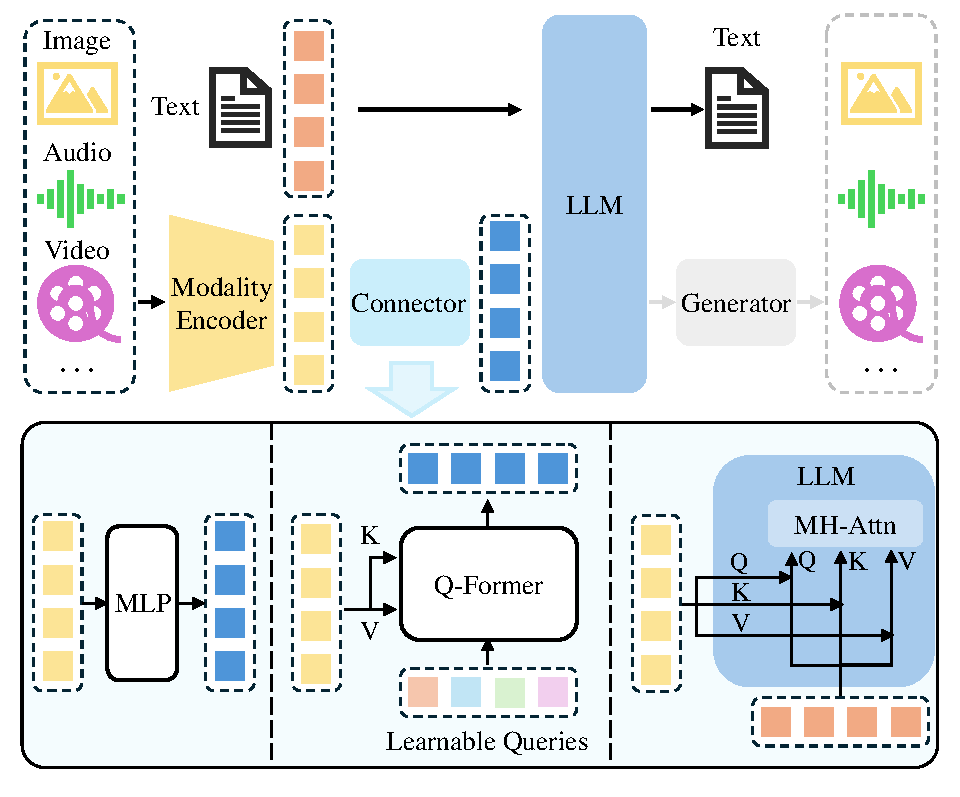
\includegraphics[width=\linewidth]{figs/survey-arch.pdf}
    \caption{An illustration of typical MLLM architecture. It includes an encoder, a connector, and a LLM. An optional generator can be attached to the LLM to generate more modalities besides text. The encoder takes in images, audios or videos and outputs features, which are processed by the connector so that the LLM can better understand. There are broadly three types of connectors: projection-based, query-based, and fusion-based connectors. The former two types adopt token-level fusion, processing features into tokens to be sent along with text tokens, while the last type enables a feature-level fusion inside the LLM.}
    \label{fig:arch}
\end{figure}

\begin{table*}[!t]
\centering
\caption{A summary of commonly used image encoders.}
\begin{tabular}{lcccc}
\toprule
\textbf{Variants} & \textbf{Pretraining Corpus}            & \textbf{Resolution} & \textbf{Samples (B)} & \textbf{Parameter Size (M)} \\ \midrule
OpenCLIP-ConvNext-L~\cite{cherti2023reproducible}     & LAION-2B     & 320 & 29 & 197.4  \\ 
CLIP-ViT-L/14~\cite{clip}           & OpenAI's WIT & 224/336 & 13 & 304.0  \\ 
EVA-CLIP-ViT-G/14~\cite{sun2023eva} & \multicolumn{1}{l}{LAION-2B,COYO-700M} & 224               & 11                         & 1000.0                      \\
 
OpenCLIP-ViT-G/14~\cite{cherti2023reproducible}       & LAION-2B     & 224 & 34 & 1012.7 \\ 
OpenCLIP-ViT-bigG/14~\cite{cherti2023reproducible}    & LAION-2B     & 224 & 34 & 1844.9 \\  \bottomrule
\end{tabular}
\label{tab:encoder}
\end{table*}

\subsection{Modality encoder}
The encoders compress raw information, such as images or audio, into a more compact representation.
Rather than training from scratch, a common approach is to use a pre-trained encoder that has been aligned to other modalities. For example, CLIP~\cite{clip} incorporates a visual encoder semantically aligned with the text through large-scale pre-training on image-text pairs. Therefore, it is easier to use such initially pre-aligned encoders to align with LLMs through alignment pre-training (see \S \ref{sec:train_pre_train}). 

The series of commonly used image encoders are summarized in~\cref{tab:encoder}. Apart from vanilla CLIP image encoders~\cite{clip}, some works also explore using other variants. For example, MiniGPT-4~\cite{minigpt-4} adopts an EVA-CLIP~\cite{fang2023eva,sun2023eva} (ViT-G/14) encoder, which is trained with improved training techniques.
In contrast, Osprey~\cite{yuan2023osprey} introduces a convolution-based ConvNext-L encoder~\cite{cherti2023reproducible} to utilize higher resolution and multi-level features.  
Some works also explore encoder-free architecture. For instance, the image patches of Fuyu-8b~\cite{fuyu-8b} are directly projected before sending to LLMs. Thus, the model naturally supports flexible image resolution input.

When choosing encoders, one often considers factors like resolution, parameter size, and pretraining corpus. 
Notably, many works have empirically verified that using higher resolution can achieve remarkable performance gains~\cite{bai2023qwen,liu2023improved,li2023monkey,mckinzie2024mm1}. The approaches for scaling up input resolution can be categorized into direct scaling and patch-division methods. 
The direct scaling way inputs images of higher resolutions to the encoder, which often involves further tuning the encoder~\cite{bai2023qwen} or replacing a pre-trained encoder with higher resolution~\cite{liu2023improved}. Similarly, CogAgent~\cite{hong2023cogagent} uses a dual-encoder mechanism, where two encoders process high and low-resolution images, respectively. High-resolution features are injected into the low-resolution branch through cross-attention.
Patch-division methods cut a high-resolution image into patches and reuse the low-resolution encoder. For example, Monkey~\cite{li2023monkey} and SPHINX~\cite{lin2023sphinx} divide a large image into smaller patches and send sub-images together with a downsampled high-resolution image to the image encoder, where the sub-images and the low-resolution image capture local and global features, respectively. 
In contrast, parameter size and training data composition are of less importance compared with input resolution, found by empirical studies~\cite{mckinzie2024mm1}.

Similar encoders are also available for other modalities. For example, Pengi~\cite{deshmukh2024pengi} uses CLAP~\cite{elizalde2023clap} model as the audio encoder. ImageBind-LLM~\cite{han2023imagebind} uses the ImageBind~\cite{girdhar2023imagebind} encoder, which supports encoding image, text, audio, depth, thermal, and Inertial Measurement Unit (IMU) data. Equipped with the strong encoder, ImageBind-LLM can respond to the input of multiple modalities. 



\begin{table*}[!t]
\centering
\caption{A summary of commonly used open-sourced LLMs. en, zh, fr, and de stand for English, Chinese, French, and German, respectively.}
\label{tab:llm}
\begin{tabular}{lccccc}
\toprule
\textbf{Model} & \textbf{Release Date} & \textbf{Pretrain Data Scale} & \textbf{Parameter Size  (B)} & \textbf{Language Support} & \textbf{Architecture} \\
\midrule
Flan-T5-XL/XXL~\cite{chung2022scaling} & Oct-2022 & -           & 3/ 11           & en, fr, de & Encoder-Decoder \\
LLaMA~\cite{llama}          & Feb-2023 & 1.4T tokens & 7/ 13/ 33/ 65   & en         & Causal Decoder  \\
Vicuna~\cite{vicuna}         & Mar-2023 & 1.4T tokens & 7/ 13/ 33       & en         & Causal Decoder  \\
LLaMA-2~\cite{llama-2}        & Jul-2023 & 2T tokens   & 7/ 13/ 70       & en         & Causal Decoder  \\
Qwen~\cite{qwen-lm}           & Sep-2023 & 3T tokens   & 1.8 / 7/ 14/ 72 & en, zh     & Causal Decoder  \\
\bottomrule
\end{tabular}
\end{table*}

\subsection{Pre-trained LLM}
Instead of training an LLM from scratch, it is more efficient and practical to start with a pre-trained one. Through tremendous pre-training on web corpus, LLMs have been embedded with rich world knowledge, and demonstrate strong generalization and reasoning capabilities. 

We summarize the commonly used and publicly available LLMs in~\cref{tab:llm}. Notably, most LLMs fall in the causal decoder category, following GPT-3~\cite{brown2020language}. Among them, Flan-T5~\cite{chung2022scaling} series are relatively early LLMs used in works like BLIP-2~\cite{li2023blip} and InstructBLIP~\cite{instructblip}. LLaMA series~\cite{llama,llama-2} and Vicuna family~\cite{vicuna} are representative open-sourced LLMs that have attracted much academic attention. Since the two LLMs are predominantly pre-trained on English corpus, they are limited in multi-language support, such as Chinese. In contrast, Qwen~\cite{qwen-lm} is a bilingual LLM that supports Chinese and English well. 

It should be noted that scaling up the parameter size of LLMs also brings additional gains, similar to the case of increasing input resolution. Specifically, Liu \etal \cite{liu2023improved, liu2024llavanext} find that simply scaling up LLM from 7B to 13B brings comprehensive improvement on various benchmarks. Furthermore, when using a 34B LLM, the model shows emergent zero-shot Chinese capability, given that only English multimodal data are used during training. Lu~\etal~\cite{lu2023empirical} see a similar phenomenon by scaling up LLMs from 13B to 35B and 65B/70B, where the larger model size brings consistent gains on benchmarks specifically designed for MLLMs. 
There are also works that use smaller LLMs to facilitate deployment on mobile devices. For example, MobileVLM series~\cite{chu2023mobilevlm,chu2024mobilevlm} use downscaled LLaMA~\cite{llama} (termed as MobileLLaMA 1.4B/2.7B), enabling efficient inference on mobile processors.

Recently, explorations of Mixture of Experts (MoE) architecture for LLMs have garnered rising attention~\cite{shen2023mixture,jiang2024mixtral,fedus2022switch}. Compared with dense models, the sparse architecture enables scaling up total parameter size without increasing computational cost, by selective activation of the parameters. Empirically, MM1~\cite{mckinzie2024mm1} and MoE-LLaVA~\cite{lin2024moe} find that MoE implementation achieves better performance than the dense counterpart on almost all the benchmarks.



\subsection{Modality interface}
\label{sec:arch_modality_interface}
Since LLMs can only perceive text, bridging the gap between natural language and other modalities is necessary. 
However, it would be costly to train a large multimodal model in an end-to-end manner.  
A more practical way is to introduce a learnable connector between the pre-trained visual encoder and LLM. 
The other approach is to translate images into languages with the help of expert models, and then send the language to LLM.


\noindent \textbf{Learnable Connector.}
It is responsible for bridging the gap between different modalities.
Specifically, the module projects information into the space that LLM can understand efficiently. 
Based on how multimodal information is fused, there are broadly two ways to implement such interfaces, \ie token-level and feature-level fusion.

For token-level fusion, features output from encoders are transformed into tokens and concatenated with text tokens before being sent into LLMs. A common and feasible solution is to leverage a group of learnable query tokens to extract information in a query-based manner~\cite{carion2020end}, which first has been implemented in BLIP-2~\cite{li2023blip}, and subsequently inherited by a variety of work~\cite{x-llm, instructblip, video-llama}. Such Q-Former-style approaches compress visual tokens into a smaller number of representation vectors.
In contrast, some methods simply use a MLP-based interface to bridge the modality gap~\cite{llava, pmc-vqa, pandagpt, detgpt}. 
For example, LLaVA series adopts one/two linear MLP~\cite{llava, liu2023improved} to project visual tokens and align the feature dimension with word embeddings.

On a related note, MM1~\cite{mckinzie2024mm1} has ablated on design choices on the connector and found that for token-level fusion, the type of modality adapter is far less important than the number of visual tokens and input resolution. 
Nevertheless, Zeng~\etal~\cite{zeng2023matters} compare the performance of token and feature-level fusion, and empirically reveal that the token-level fusion variant performs better in terms of VQA benchmarks. Regarding the performance gap, the authors suggest that cross-attention models might require a more complicated hyper-parameter searching process to achieve comparable performance. 

As another line, feature-level fusion inserts extra modules that enable deep interaction and fusion between text features and visual features. For example, Flamingo~\cite{alayrac2022flamingo} inserts extra cross-attention layers between frozen Transformer layers of LLMs, thereby augmenting language features with external visual cues. Similarly, CogVLM~\cite{wang2023cogvlm} plugs in a visual expert module in each Transformer layer to enable dual interaction and fusion between vision and language features. For better performance, the QKV weight matrix of the introduced module is initialized from the pre-trained LLM.
Similarly, LLaMA-Adapter~\cite{llama-adapter} introduces learnable prompts into Transformer layers. These prompts are first embedded with visual knowledge and then concatenated with text features as prefixes.

In terms of parameter size, learnable interfaces generally comprise a small portion compared with encoders and LLMs. Take Qwen-VL~\cite{bai2023qwen} as an example, the parameter size of the Q-Former is about 0.08B, accounting for less than 1\% of the whole parameters, while the encoder and the LLM account for about 19.8\% (1.9B) and 80.2\% (7.7B), respectively.

\noindent \textbf{Expert Model.}
Apart from the learnable interface, using expert models, such as an image captioning model, is also a feasible way to bridge the modality gap~\cite{yin2023woodpecker,guo2023images,CAT,chatcaptioner}.
The basic idea is to convert multimodal inputs into languages without training.
In this way, LLMs can understand multimodality by the converted languages.
For example, VideoChat-Text~\cite{videochat} uses pre-trained vision models to extract visual information such as actions and enriches the descriptions using a speech recognition model. 
Though using expert models is straightforward, it may not be as flexible as adopting a learnable interface. The conversion of foreign modalities into text would cause information loss. For example, transforming videos into textual descriptions distorts spatial-temporal relationships~\cite{videochat}.

